It is necessary here to briefly examine what money actually is in the world outside of metaverses, so we can understand it in the context of a virtual global space. In the previous section Bitcoin can be viewed in a couple of different lights. As a self custody digital bearer asset it can be viewed as `property', like gold, i.e. not a liability on someone else's asset sheet. Indeed this has long been one of the assertions of the community and it finds favour in law, \href{https://www.regulationasia.com/shanghai-court-says-bitcoin-is-protected-by-law-as-virtual-property/}{possible most ironically in China} which of course banned mining. `Money' though is a far more \href{https://www.bankofengland.co.uk/knowledgebank/what-is-money}{slippery concept} to grasp. It seems very likely that Bitcoin is evolving as a ``base money'', and it's important to define that, but there are many other kinds of money within the online world which can potentially transfer value within virtual social spaces.
\section{Defining money}
Money is an economic good, that is generally accepted as a medium of exchange. This simple and specific description doesn't do justice to the complexity of everything that humans consider to be money. Even the Encyclopaedia Britannica strays from this immediately in their definition:\par
\textit{``money, a commodity accepted by general consent as a medium of economic exchange. It is the medium in which prices and values are expressed; as currency, it circulates anonymously from person to person and country to country, thus facilitating trade, and it is the principal measure of wealth.''}. \\
In which it can be seen that the principle measure of wealth might not be money at all, but rather property, credit, etc. So are these things money? Is a promise on a ledger money? The assertion at the top of this section is challenged by different schools of economic thinking. Global debt is around an order of magnitude larger than base money, and most wealth is stored in illiquid land/built environment (some \$300T), and yet the system seems to work fine. The debt theory of money offered by anthropologist David Graeber suggests that money is an abstraction of barter, and thereby `credit', but credit clearly pre-dates money, and needs no barter, commodity, intermediary nor underlying asset \cite{homer1996history}. This suggests that money is something slightly different.\par
Money seems to have evolved for two principle purposes; trade outside of a village context, and inheritance \cite{szabo2002shelling}. In doing this it somewhat replaced and augmenting `credit', which as said above, was a promise between parties based on future actions, and likely as old as rudimentary language itself.\par
Money can be divided into two categories, which are fungible (interchangeable) from the point of view of the users. Base money is `commodity' money which is backed by assets, or tangible physical (or digital) goods through the actions of a central bank ledger, and is around \$30-\$40T. Everything else is `fiduciary media' \cite{selgin1996defense}.\par
All fiduciary money is credit but not all credit is fiduciary money. Nobody knows the extent of the global supply of fiduciary media. It encapsulates all the new digital money platforms like PayPal, gift cards, offshore accounts and all manner of other vehicles, and is thought to be many tens of trillions of pounds. This somewhat muddies the waters since money that is backed by `something' blends away into money which cannot reasonably be assayed. This in turn undermines the assertion that money is backed. It seems that a combination of available raw materials and labour, central banks and their associated political structures \cite{barsky1987fisher}, and global markets drive the value of money up and down relative to ``stuff'' in the shops. This manifests as `inflation', which is `possibly' the effect of not pegging money to an asset such as silver, or gold as in the past \cite{hall2009inflation}. While the gross drivers of inflation seems to be accepted and understood, nobody \href{https://www.dailymail.co.uk/news/article-10966165/Jerome-Powell-admits-understand-better-little-understand-inflation.html}{seems very sure} how the \href{https://www.bloomberg.com/opinion/articles/2022-08-19/this-economy-is-proving-too-complicated-for-economists}{various aspects interact}.It may be that central banks actually have no decent response to global monetary pressures and are overdue a paradigm shift, as \href{https://www.ft.com/content/2d79d153-fffa-4441-b79f-0a808a51108f}{explained by Daniela Gabor} (Professor of economics and macrofinance at UWE Bristol):\\ 
\textit{``...last stage of a central banking paradigm, when it implodes under the contradictions of its class politics? Under the financial capitalism supercycle of the past decades, inflation-targeting central banks have been outposts of (financial) capital in the state, guardians of a distributional status-quo that destroyed workers’ collective power while building safety nets for shadow banking.\\
The limits of this institutional arrangement that concentrates (pricing) power and profit in (a few) corporate hands are now plain to see. If the climate and geopolitical of 2022 are omens of Isabel Schnabel’s Great Volatility that most central banks and pundits expect for the near future, then macro-financial stability requires new framework for co-ordination between central banks and Treasuries that can support a state more willing to, and capable of, disciplining capital.\\
But such a framework would threaten the privileged position that central banks have had in the macro-financial architecture and in our macroeconomic models. The history of central banking teaches us that policy paradigms die when they cannot offer a useful framework for stabilising macroeconomic conditions, but never at the hands of central bankers themselves.''}\par
All this makes it \href{https://www.lynalden.com/what-is-money/}{hard to find} a universally accepted and explicable definition of money. The best approach may be to look at the properties of a thing which is asserted to be a money. In his book `A history of money', Glyn Davies identifies ``cognisability, utility,  portability, divisibility, indestructibility, stability of value, and homogeneity'' \cite{davies2010history}.\par
Stroukal examines Bitcoins' likely value as a money from an Austrian economics perspective and identifies ``portability, storability, divisibility, recognizability, homogeneity and scarcity'' \cite{stroukal2018can}.\par
A helpfully brief and useful \href{http://money.visualcapitalist.com/infographic-the-properties-of-money/}{web page by Desjardins from 2015} describes some properties and explains them in layman's terms below:
\begin{itemize}
\item Divisible: Can be divided into smaller units of value.
\item Fungible: One unit is viewed as interchangeable with another.
\item Portable: Individuals can carry money with them and transfer it to others.
\item Durable: An item must be able to withstand being used repeatedly.
\item Acceptable: Everyone must be able to use the money for transactions.
\item Uniform: All versions of the same denomination must have the same purchasing power.
\item Limited in Supply: The supply of money in circulation ensures values remain relatively constant.
\end{itemize}
\subsection{Global currency interactions}
The legacy moniker ``third world'' came from a division of the world along economic lines \cite{tomlinson2003third}. At the time this was the petrodollar / neo-institutional hegemony \cite{caballero2008financial, spiro2019hidden}, vs the economic superpower of the soviet block, and then `the rest'; unaligned economic powers.\par
This old framework has fallen away with the associated terminology, but it's useful to look at what money `is' from a global viewpoint, because all money is effectively trust in the liability held by some defined counter party.\par
Right now the dollar system is still predominant, but it seems likely that there are new axes forming, especially around the \href{https://www.wsj.com/articles/saudi-arabia-considers-accepting-yuan-instead-of-dollars-for-chinese-oil-sales-11647351541}{Chinese Yuan}. It's clear that central banks have been aware of this potential transition away from a global dollar / energy system. The Dollar has potentially suffered from the radical expansion of the money supply over the last 70 years or so under the private ``Eurodollar'' system \cite{grewal2020struggling}. Some policy makers have been looking back to the great economist John Maynard Keynes' ideas for a neutral basket of assets as a global synthetic hedgemonic currency \cite{carney2019growing, piffaretti2009reshaping} which would almost certainly consist partly of gold \cite{stoeferle2018gold}.\par
Use of the dollar system has recently been shown more and more to be contingent on adherence to US defined political principles. This is evidenced most starkly by the seizure of Russian central bank \href{https://twitter.com/RussianEmbassy/status/1504530573527760909}{foreign reserves}, a new and untried projection of monetary power.\par  
The Chinese Yuan/Renminbi is potentially stepping in where the petrodollar is now waning \cite{mathews2018china}. The effects of this expansion of economic influence by China, through a potential petro-Yuan, and the belt and road initiative \cite{huang2016understanding}, are not yet felt, but the lines are fairly clearly defined and may be felt over the coming decades. The Euro system is potentially even less stable because of recent energy supply pressures, and \href{https://www.fitchratings.com/research/sovereigns/energy-crisis-increases-fiscal-risks-to-western-europe-sovereigns-23-09-2022}{internal tensions} in the bond markets. Though it seems to be less `weaponised', it comes with it's own restrictions for use, especially through the International Monetary Fund (IMF). It is notable for instance that the IMF have included a clause in their negotiations with Argentina to `discourage' the use of crypto based money, leading to a complete ban on banks offering the products only days after they began. This is likely a response to the adoption of Bitcoin by El Salvador, something with which the IMF is very uncomfortable. They are also wary of the ability of nation states to \href{https://www.imf.org/en/Publications/GFSR/Issues/2022/04/19/global-financial-stability-report-april-2022}{monetise their energy reserves} without the need for export markets. They do however \href{https://blogs.imf.org/2022/06/16/how-crypto-and-cbdcs-can-use-less-energy-than-existing-payment-systems/}{concede that CBDCs and `some' crypto assets} may be more energy efficient than traditional systems. It seems to industry insiders that they are learning in public.\par
The new `third world' who are excluded from the Dollar and/or Yuan poles of the global economy might drift toward the `basket of assets' discussed by Keynes and Carney above. As mentioned this will certainly have a component of gold, and likely other commodity assets such as rare metals. For our purposes here it's also possible that there would be a small `hedge' allocation of Bitcoin or \href{https://www.independent.co.uk/tech/bitcoin-el-salvador-crypto-btc-b2079881.html}{even a global axis} of `unaligned' nations using the asset \cite{hendrickson2021value}. Block and Wakefield research \href{https://block.xyz/2022/btc-report.pdf}{found that in developed nations} Bitcoin is treated as in investment, while in less wealthy demographics there is interest in the utility. This is evidenced in the early nation state adoption seen and described to date, and the game theory incentive explained by Fidelity in the introduction. It's too early to tell if this `unaligned money' could constitute a global economic pole, but it's interesting that some commentators are now even discussing this, and that \href{https://docs.google.com/document/d/1Ynl5bbdTqev-wbTAWQoeWdh1cJVf3ortuSjre9K9wGQ/edit}{carbon neutrality research} is being undertaken specifically for this application.

\section{International money transfer networks}
Transferring money from one financial jurisdiction to another is itself a global marketplace which has accreted over the entire course of human history. It's far less useful here to discuss the mythos of salt and seashells as a mechanisms of international remittance and taxation \cite{gainsford2017salt, goldberg2005famous}. Suffice it to say that there are dozens, if not hundreds, of cross border payment companies who make their business from taking a percentage cut of an international money transfer. There are also hundreds if not thousands of banks who offer this service as part of their core business portfolio. This section looks at some of the major players, and their mechanism, to contextualise the more recent shifts brought about by technology.
\subsection{Swift, ISO 20022, and correspondence banking}
Society for Worldwide Interbank Financial Communiactions (SWIFT) was initially formed in 1973 between 239 banks across 15 countries. They needed a way to improve handling of cross border payments. It is now the global \href{https://www.swift.com/standards}{standard} for financial message exchange in over 200 countries, and has recently found itself under a fresh spotlight, during the invasion of Ukraine. The system handles around 40 million short, secure, code transmissions a day, which represent crucial data about a transaction and the parties involved. It is used by both banks and major financial institutions to speed up settlement between themselves, on behalf of the clients and customers. It replaced the Telex (wire transfer) system. The new proposed and incoming standard to replace SWIFT is \href{https://www.swift.com/standards/iso-20022}{ISO20022} which is a complex and data rich arrangement. To be clear the SWIFT consortium are promoting this new standard to their 11,000 plus global user base, and there is significant investment and hype from major financial players, but it seems unclear what the actual take-up will or even should be. A group of `crytocurrencies' are heavily involved in the ISO20022 standard, and there's been experimentation with private permissioned distributed ledger technologies. It's actually somewhat unclear what value they bring, and possible that the relationship of these public ledgers to international bank to bank messaging is a marketing distraction. Note that SWIFT, ISO20022, and the associated tokens within crypto are all themselves products which have a business model. They are all intermediaries which will demand a mediating fee somewhere. All of this proposed functionality could be replaced by central bank digital currencies, which will be discussed later in the section.
\subsection{VISA and Mastercard}
Both major credit card companies are building out their ``crypto'' capabilities. Mastercard have \href{https://finance.yahoo.com/news/mastercard-crypto-secure-200559003.html}{launched a back end platform} to mitigate fraud when buying digital products with their cards. VISA have announced a ``\href{https://investor.visa.com/news/news-details/2021/Visa-Introduces-Crypto-Advisory-Services-to-Help-Partners-Navigate-a-New-Era-of-Money-Movement/default.aspx}{crypto business to business support unit}''. They have also \href{https://www.cnbc.com/2022/10/07/visa-partners-with-ftx-in-a-bet-that-shoppers-still-want-to-spend-cryptocurrencies-in-a-bear-market.html}{partnered with crypto exchange FTX} to allow users to spend digital assets directly using their VISA cards.
\subsection{Money transfer operators}

\href{https://www.toptal.com/finance/market-research-analysts/international-money-transfer}{International Money Transfer Operators analysis}

western union etc, moneygram, transferwise,
\subsection{Digital disruptive fintech}
It seems that the neobank providers of digital banking apps are likely to converge with native digital asset ``wallets''. This is also the thesis advanced by the Ark intestments Big Ideas paper.\par
CNN have a \href{https://money.cnn.com/infographic/technology/mobile-payment-comparison/index.html}{useful primer} of the most prevalent mobile digital payment methods. This can be seen in Figure \ref{fig:CNNmobile}.
\begin{figure}
  \centering
    \includegraphics[width=\linewidth]{CNNmobile}
  \caption{Comparison of mobile based payment systems}
  \label{fig:CNNmobile}
\end{figure}
This comparison makes it pretty clear that Bitcoin is not ready as a personal mobile payment system. That's not to say that there isn't a place for the underlying technology in global payment processing. 
The most interesting example of this is Strike, a product in the international fintech arena. It is a `global' money transmitter which uses bank connections in local currencies, but a private version of the Lightning network with settlement on the Bitcoin main chain. In practice users connect the app to their bank and can send money to the bank connected Strike app of another user instantly, and without a fee. This is a far better product than those previously available. In principle it's open API allows many more applications to be integrated into the Strike back end. Twitter already uses this for international tipping (and remittance). It seems that this is a perfect contender for supporting transactions in open metaverse applications, and that may be true, but Strike is currently only available in three countries (USA, El Salvador, Argentina).\par
Paypal, xoom, Strike, servicing smaller payments, cashapp, venmo, revulot, 
Paypal especially is noteworthy for their recent Orwellian gaffe suggesting in their terms and conditions that they would be able to fine users \$2500 for ``disseminating informational''. They \href{https://www.yahoo.com/video/paypal-policy-permits-company-fine-143946902.html}{quickly walked this back} but this kind of private fintech action is highly suggestive of a need for uncensorable money such as Bitcoin.
\subsection{Stablecoins}
Stablecoins are `crypto like' instruments which are `pegged' at a 1:1 ratio with nationally issued Fiat currencies. In fact they usually correspond to units of privately issued  debt underwritten by a variety of different assets. This is (depending on the issuing company's model) a \href{https://www.americanbanker.com/opinion/ststablecoins-are-backed-by-reserves-give-us-a-break}{far more risky} unit of money than the nominal currency that they represent, but they offer significant utility. They allow the user to self custody the cryptographic bearer instrument representing the money themselves, as with blockchain. This may afford the user less friction in that they can transmit the instrument through the newer financial rails which are emerging. Once again, this is likely a product most useful to \href{https://www.cigionline.org/articles/the-future-of-fintech-is-unfolding-in-africa/?}{emerging markets}, those living under oppressive regimes, currencies \href{https://www.bloomberg.com/news/articles/2022-07-03/argentines-seek-hedging-in-crypto-after-economy-minister-resigns}{suffering from high inflation}, and countries who rely on the dollar as their currency, and within digitally native metaverse applications. These are \textit{enormous} global uses though. The use in the west is prominently for `traders' on exchanges at this time. /par
The caveat of such products is that such `units' of money can be frozen by the issuer, and they are subject to the third party risk of the issuer defaulting on the underlying instrument, instantly wiping out the value.\par
Klages-Mundt et al. wrote a paper in 2020, which explains the details of the different mechanisms and risks.\par
The following text paraphrases Spencer noon of on-chain analytics company ``OurNetwork'', who provides an \href{https://twitter.com/spencernoon/status/1524752048121466883}{useful summary} of the paper.
\textit{There are two major classes of stablecoins:
\begin{itemize}
\item Custodial: entrusted by off-chain collateral assets like fiat dollars that sit in a bank. Requires trust in third party.
\item Non-custodial (aka decentralized): fully on-chain and backed by smart contracts \& economics. No trusted parties.
\end{itemize}
In custodial stablecoins, custodians hold a combination of assets (currencies, bonds, commodities, etc.) off-chain, allowing issuers (possibly the same entity) to offer digital tokens of an reserve asset. The top 2 custodial stablecoins today are USDT and USDC.
There are 3 types of custodial stablecoins.
\begin{itemize}
\item Reserve Fund: 100\% reserve ratio. Each stablecoin is backed by a unit of the reserve asset held by the custodian. A useful example of this the \href{https://www.americanbanker.com/news/bank-stablecoin-consortium-usdf-gets-a-ceo-grows-to-9-members}{USDF banking consortium}.
\item Fractional Reserve Fund: The stablecoin is backed by a mix of both reserve assets and other capital assets.
\item Central Bank Digital Currency (CBDC): A digital form of central bank money that is widely available to the general public. CBDCs are in their nascency as today only 9 countries/territories have launched them, many of them small.
\end{itemize}
Custodial stablecoins have three major risks:
\begin{itemize}
\item Counterparty Risk (fraud, theft, govt seizure, etc.)
\item Censorship Risk (operations blocked by regulators, etc.)
\item Economic Risk (off-chain assets go down in value)
\end{itemize}
Each can result in the stablecoin value going to zero.}\par
It's worth taking a look at these tokens individually, to get a feel for the trade-offs, and figure out how they might be useful for us in our proposed metaverse applications. It's important to know that these tokenised dollars and/or other currencies are issued on top of the public blockchains we have been detailing throughout. Which tokens are on what blockchains is constantly evolving, so it's not really worth enumerating specifics. In a metaverse application it would be necessary to manage both the underlying public blockchain and the stablecoin issued on top of it, making the interaction with the global financial system perversely more not less complex. In the following list of a few of the major coins, the first hyperlink is the whitepaper if it's available.
\begin{itemize}
\item \href{https://f.hubspotusercontent30.net/hubfs/9304636/PDF/centre-whitepaper.pdf}{USDC} is a dollar backed coin issued by a consortium of major players in the space, most notably Circle, and Coinbase. It's has a better transparency record than tether but is still not backed 1:1 by actual dollars in reserve. It may or may not be a fractional reserve asset. It's  well positioned to take advantage of regulatory changes in the USA, and seems to be quietly lobbying to be the choice of a government endorsed digital dollar, at least a significant part of a central bank digital currency initiative. It's too early to tell how this will work out, but it has \href{https://www.forbes.com/sites/ninabambysheva/2022/04/13/blackrocks-newest-investment-paves-the-way-for-digital-assets-on-wall-street/?}{substantial `legacy finance backing'}. It is the only stablecoin to increase slightly in value (depegging upward) in the wake of the UST implosion. This `flight to quality' shows the advantage of the work that CENTRE put into regulatory compliance. It runs on Ethereum, Algorand, Solana, Stellar, Tron, Hedera, Avalanche and Flow blockchains. At this time USDC may be \href{https://twitter.com/Excellion/status/1567472488589963264}{under speculative attack} by Chinese exchange Binance, in favour of their own offering BUSD, and is losing market share. 
\item Binance USD is the dollar equivalent token from global crypto exchange behemoth Binance. It's released in partnership with Paxos, who have a strong record for compliance, and transparency. Paxos also offer USDP. Both these stablecoins claim to be 100\% backed by dollars, or US treasuries. They are regulated under the more restrictive New York state financial services and have a monthly \href{https://paxos.com/attestations/}{attestation report}.
\item \href{https://makerdao.com/en/whitepaper#abstract}{MakerDAO Dai} is an Ethereum based stablecoin and one of the older offerings. It's been `governed' by a DAO since 2014. `Excess collateral', above the value of the dai-dollars to be minted, is voted upon before being committed to the systems' cryptographic `vaults' as a backing for the currency. These dai can then be used across the Ethereum network. Despite the problems with DAOs, and the problems with Ethereum, DAI is well liked by its community of users and has a healthy billion dollars of issuance. They may be \href{https://thedefiant.io/tornado-impact-makerdao-dai}{dangerously exposed} to the new crackdown in the USA, and there is \href{https://twitter.com/bantg/status/1557733094899138560}{internal talk} of pro-actively abandoning DAI altogether.
\item \href{https://trueusd.com/pdf/TUSD_WhitePaper.pdf}{TrueUSD} claims to be fully backed by US dollars, held in escrow. It runs on the Ethereum blockchain. They have attestation reports \href{https://real-time-attest.trustexplorer.io/truecurrencies}{available on demand} and claim fully insured deposits. It's not quite that simple in that a portion of the backing is `cash equivalents'.
\item \href{https://www.gemini.com/static/dollar/gemini-dollar-whitepaper.pdf}{Gemini GUSD} claim reserves are ``held and maintained at State Street Bank and Trust Company and within a money market fund managed by Goldman Sachs Asset Management, invested only in U.S. Treasury obligations.'' which seems pretty clear.
\item \href{https://assets.website-files.com/611153e7af981472d8da199c/618b02d13e938ae1f8ad1e45_Terra_White_paper.pdf}{TerraUSD} (UST) \textbf{was} a newer and more experimental stablecoin, and one of a set of currency representations within the network. It worked in concert with the LUNA token on the Cosmos blockchain in order to keep it's dollar stability. It was not backed in the same way as the other tokens, instead relying on an arbitrage mechanism using LUNA. In essence the protocol paid users to destroy LUNA and mint UST when the price was above one dollar, and vice versa. This theoretically maintained the dollar peg. There was much concern that this model of \href{https://mirror.xyz/damsondao.eth/OVeBrmrfcWm7uKLlA2Q4W1XTVkFU3cMKfNWhgf7mQuM}{`algorithmic stable coin'} is unstable \cite{clements2021built}. The developers of the Terra tried to address this concern by \href{https://etherscan.io/address/0xad41bd1cf3fd753017ef5c0da8df31a3074ea1ea}{buying enormous amounts} of Bitcoin, which they quickly had to employ to address UST drifting downward from \$1. This failed to address the `great depegging', with LUNA crashing to essentially zero, destroying some \$50B of capital. It will now likely act as a cautionary tale to other institutions considering Bitcoin as a `reserve asset'. An \href{https://github.com/GMCyberFoundry/Metaverse/blob/b06547bf290392d2ff02e5142dae7386d888a9de/Book/04_money.tex#L186}{earlier version of this book} highlighted the specific variation of the risk which quickly manifested.
\item \href{https://tether.to/en/whitepaper/}{Tether} is the largest of the stablecoins, with some \$70B in circulation, and the third largest `crypto'. This has been a meteoric rise, attracting the ire and scrutiny of \href{https://www.cftc.gov/PressRoom/PressReleases/8450-21}{regulators} and \href{https://www.bloomberg.com/news/features/2021-10-07/crypto-mystery-where-s-the-69-billion-backing-the-stablecoin-tether}{investigators}. There was considerable doubt that Tether had sufficient assets backing their synthetic dollars, but the market seems not to mind. Recently however they have transitioned to being backed by US treasury bills, a perfect asset for this use case. It's resilience against `bank runs' was tested in May 2022 when \$9B was redeemed directly for dollars in a few days following the UST crash (more on this later). They are \href{https://tether.to/en/tether-to-launch-gbpt-tether-tokens-pegged-to-the-british-pound-sterling/}{shortly to launch} a GBP version for the UK. It's an important technology for this metaverse conversation because of intersections with Bitcoin through the Lightning network. Tether might actually provide everything needed. It's only as safe as the trust invested in the central issuer though, and we will employ the asset through the Taro technology described earlier, but it's notable and somewhat ironic that it's obviously better and more transparently backed than most banks and probably all novel fiat fintech products.
\end{itemize}  .
\subsubsection{The evolving US position}
In most regards the legislative front line is happening in the USA. Treasury Secretary Yellen responded to the collapse of Terra/UST \href{https://www.youtube.com/watch?v=kU0xYBRfgvU}{saying that}: \textit{``A comprehensive regulatory framework for US dollar stablecoins is needed''}. She also said that the stablecoin market is too small to pose systemic risk at this time. This is clearly an evolving situation, but the incredible consumer exposure to these risky products is likely to elicit a swift and significant response, and the timing seems right for intervention. The markets suggest that USDC will be the eventual winner.\par Koning meanwhile has looked into the different \href{http://jpkoning.blogspot.com/2021/08/stablecoin-regulatory-strategies.html}{regulatory approaches} used by various stablecoins.\par
\begin{itemize}
\item The highly regulated New York state financial framework (Paxos, Gemini)
\item Piggyback off of a (Nevada) state-chartered trust [TrueUSD, HUSD]
\item Get dozens of money transmitter licenses [USDC]
\item Stay offshore [Tether]
\end{itemize}

\href{https://www.americanbanker.com/news/toomey-unveils-stablecoin-bill-granting-occ-authority-for-payments-charter}{New legislation} specific to the concept of stablecoins is now entering the system under Sen Toomey. There are many provisions in the bill, mostly pertaining to convertibility and the ever present problem of attestation of the `backing' of these products. Mention has already been made of the major bill advanced by Sen. Lummis and Gillibrand. This bill also includes significant provision around stablecoins. Lummis said \textit{``Stablecoins will have to be either FDIC insured or more than 100\% backed by hard assets.''}. This is good news for this section of the digital asssets space.\par
Crucially there is also more clarity on privacy. This is a huge threat from digital money systems, and the USA is likely to lead. Remember though that none of this is yet law.\par 
Valkenburg, the lead researcher of a US think tank in digital assets \href{https://twitter.com/valkenburgh/status/1511783339065237521}{says the following}: \textit{``Stablecoin TRUST Act, is a discussion draft mostly about stablecoins, but it also has important privacy protections for crypto users broadly: it puts real limits on warrantless surveillance by narrowing what info can be collected from third parties. Last summer we fought a provision in the infrastructure bill that damaged the privacy of crypto users by expanding the broker definition (who needs to report information about transactions to the IRS) \& crypto 6050I reporting (reports on business transactions over \$10,000). The winter before we fought and successfully delayed a rushed proposal from the outgoing Trump administration to mandate that exchanges collect information about persons who are not their customers, who hold crypto at addresses in wallets they control directly. the Stablecoin TRUST Act would stop these encroachments, constrain the treasury from collecting any nonpublic information unless they get a search warrant or collect only information voluntarily provided to an exchange by a customer and for a legitimate business purpose. If “voluntarily provided for a legitimate business purpose” sounds familiar to you, that’s b/c it's the constitutional standard articulated by the Court in Carpenter describing LIMITED circumstances where warrantless searches of customer data are ok.It’s the standard we’ve advocated must also limit warrantless data collection at crypto exchanges. If exchanges must collect information about non-customers, that information is, by definition, not voluntarily provided for a legitimate business purpose.''}


%Crypto dollarisaton (myanmar)
%\href{https://twitter.com/Stacks/status/1409996245096148998}{USDC on Bitcoin?}


%It's worth pointing out that Meta (Facebook at the time) had aspirations for a global stablecoin cryptocurrency called 
%\href{https://bitcoin-red.com/facebook-libra-the-inside-story-of-how-the-companys-cryptocurrency-dream-died/}{Libre}, 
  
%\href{https://www.usdfconsortium.com/}{USDF bank issued private dollar stablecoin}

%\href{https://www.bloomberg.com/news/articles/2022-01-07/paypal-is-exploring-launc,h-of-own-stablecoin-in-crypto-push}{Paypal}


%Whatsapp, Novi, USDP etc

\subsubsection{The evolving UK position}
As mentioned briefly in the introduction the UK has recently \href{https://www.gov.uk/government/news/government-sets-out-plan-to-make-uk-a-global-cryptoasset-technology-hub}{signalled an enthusiasm} for stablecoins as ``means of payment''. This is a stark reversal of their previous legislative momentum is possibly a response to the \href{https://www.coindesk.com/policy/2022/05/11/eu-commission-favors-ban-on-large-scale-stablecoins-document-shows/}{tightening of rhetoric} in Europe around such assets. The \href{https://publications.parliament.uk/pa/bills/cbill/58-03/0146/220146.pdf}{Financial Services and Markets Bill.} became law in July 2022. An excerpt pertaining to stablecoins can be seen in Figure \ref{fig:ukdigitalbill}. \par
The U.K. Financial Conduct Authority’s chief executive, Nikhil Rathi, outlined the FCA’s regulatory goals at the Peterson Institute for International Economics: \textit{``The U.S. and U.K. will deepen ties on crypto-asset regulation and market developments — including in relation to stablecoins and the exploration of central bank digital currencies.''} \par
The timing seems right to explore the use of stablecoins in metaverse applications up the list of choices. 

\begin{figure}
  \centering
    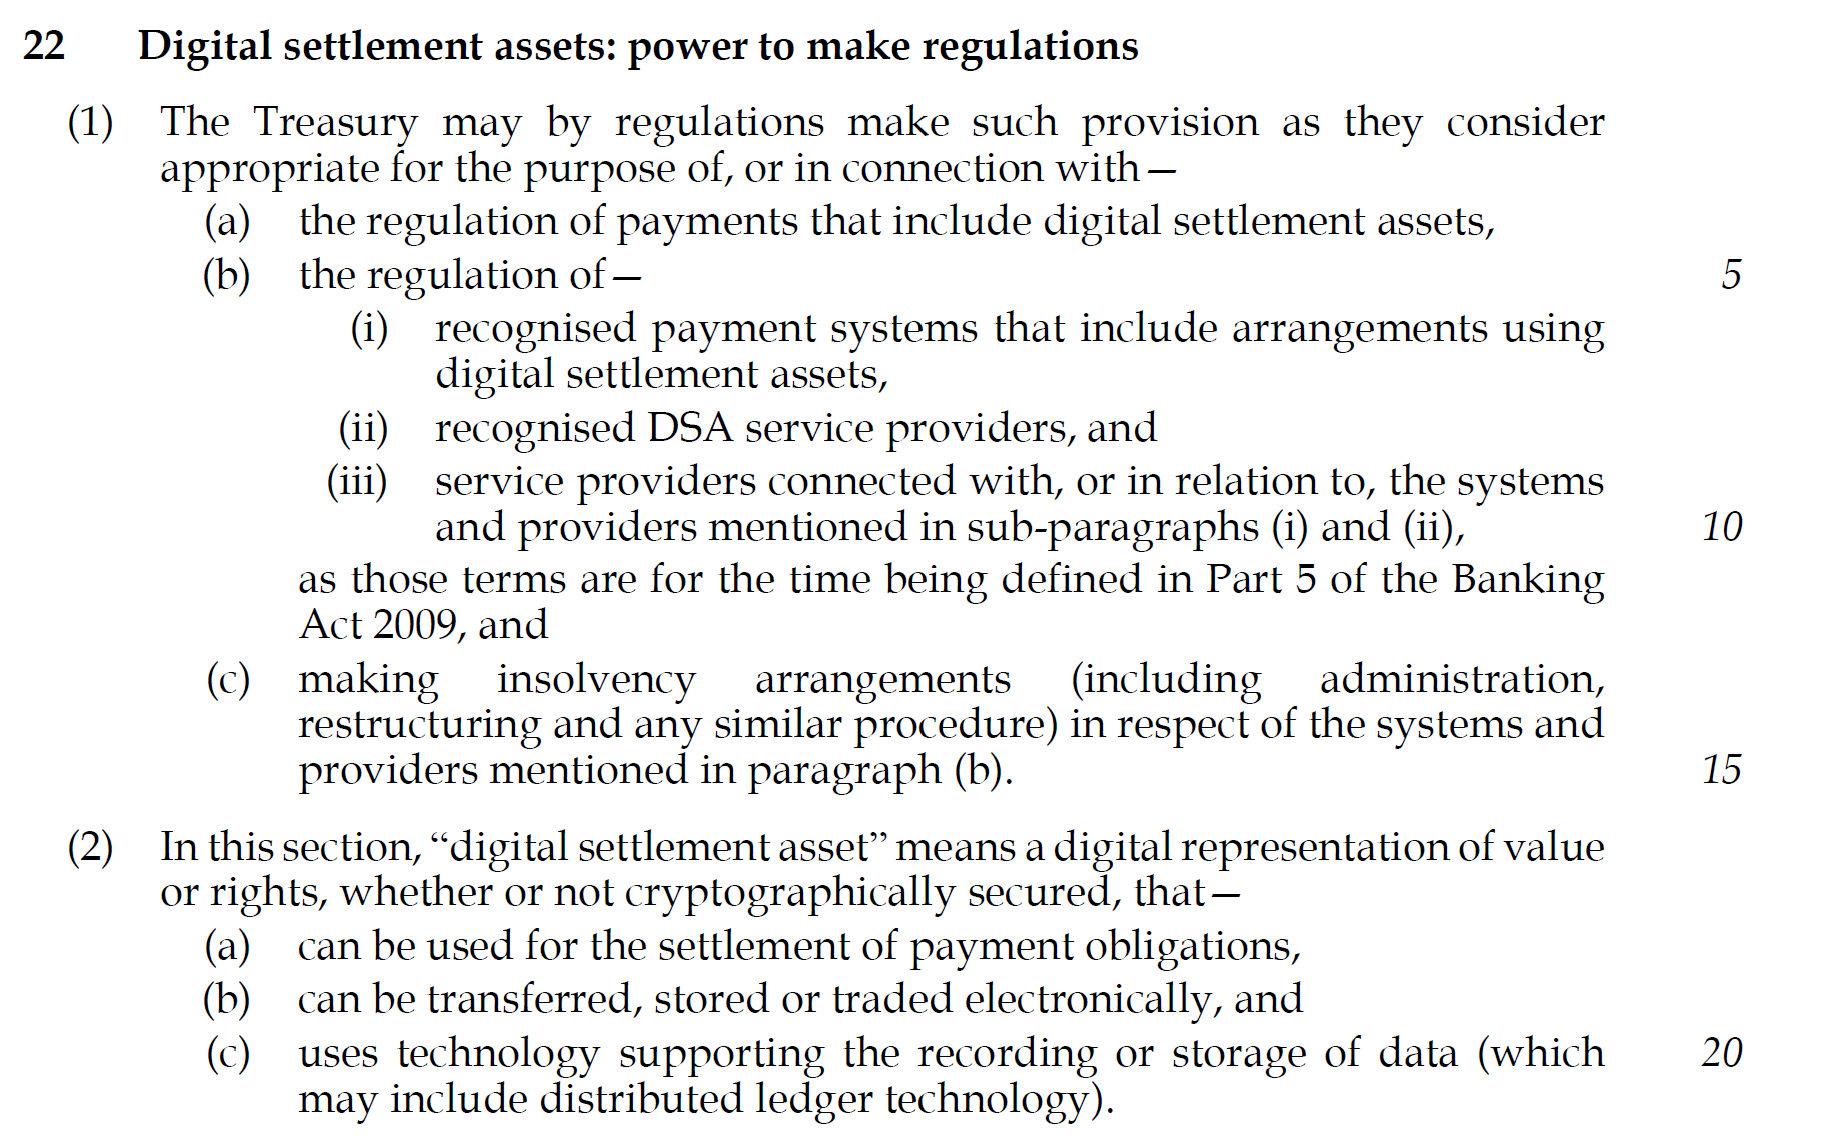
\includegraphics[width=\linewidth]{ukdigitalbill}
  \caption{The UK signs into law regulation of digital representatives of value}
  \label{fig:ukdigitalbill}
\end{figure}

\subsubsection{Stables in metaverse applications}
It makes a \textbf{lot} of sense to consider stablecoin transfer as the money in metaverses. USDC is furthest along this possible adoption curve. Their partnership with global payment provider Stripe has \href{https://stripe.com/blog/expanding-global-payouts-with-crypto}{enabled global dollar transfer} within Twitter for users of their `Connect' platform. This leverages the Polygon chain (mentioned in the blockchain chapter). Many digital wallets can be connected from the user end, with Metamask potentially being the easiest to integrate. This has also been mentioned in the book. The downside of this for our open platform is that none of these elements are particularly open, or distributed, and the users of the platform will still need to use an exchange to get the USDC to spend. This approach makes it easier for the vendors and product providers in the metaverse applications to accept USDC, but everything else is actually harder.

\section{Central bank digital currencies}
If 2022 was the year of the stablecoin then 2023 is likely to be the year of the central bank digital currency (CBDC). CBDCs would likely not exist without the 2019 catalyst of \href{https://www.thetimes.co.uk/article/facebooks-libra-cryptocurrency-project-ends-in-failure-cxvnnc3kx}{Facebook Libre} crypto currency project, which is now \href{https://fortune.com/2022/07/01/meta-novi-crypto-payments-wallet-end-september-2022/}{cancelled} and defunct, \href{https://www.theguardian.com/world/2021/jul/09/currency-and-control-why-china-wants-to-undermine-bitcoin}{pressure exerted on central banks} by the concept of Bitcoin, and the stablecoins which emerged from the technology.\par
It now seems plausible that the world is moving toward a plurality of national and private digital currencies. Figure \ref{fig:CBDClikely} from the Bank for International Settlement, shows the growing acceptance within central banks. Their 2022 annual economic report dedicates \href{https://www.bis.org/publ/arpdf/ar2022e3.pdf}{a 42 page chapter} to the subject. Hyun Song Shin, head of research at BIS said \textit{``Our broad conclusion is captured in the motto, ‘Anything that crypto can do, CBDCs can do better.``}\par
This text from the \href{https://voxeu.org/article/benefits-central-bank-digital-currency}{thinktank VoxEU} highlights the pressure on not to be \href{https://himes.house.gov/u-s-central-bank-digital-currency}{`left behind'}: \textit{``Given the rapid pace of innovations in payments technology and the proliferation of virtual currencies such as bitcoin and ethereum, it might not be prudent for central banks to be passive in their approach to CBDC. If the central bank does not produce any form of digital currency, there is a risk that it loses monetary control, with greater potential for severe economic downturns. With this in mind, central banks are moving expeditiously when they consider the adoption of CBDC.''} The Atlantic Council \href{https://www.atlanticcouncil.org/cbdctracker/}{have a website} which tracks global adoption.\par\par
\begin{figure}
  \centering
    \includegraphics[width=\linewidth]{CBDClikely}
  \caption{More than half of central banks \href{https://www.bis.org/publ/bppdf/bispap125.htm}{surveyed by the BIS} said they saw issuance of a CBDC as possible.}
  \label{fig:CBDClikely}
\end{figure}
CBDCs are wholly digital representations of national currencies, and as such are centralised database entries, endorsed and potentially issued by national governments. The \href{https://www.federalreserve.gov/publications/files/money-and-payments-20220120.pdf}{USA's whitepaper} shows the approach. Curiously only \href{https://www.sanddollar.bs/about}{The Bahamas} seem to have a successful implementation, but it is a rapidly evolving space, and many nations are now scrambling to \href{https://twitter.com/GobiernoMX/status/1476376240873517061}{catch up}. A \href{https://www.linkedin.com/feed/update/urn:li:activity:6980330210030145536/}{post on the LinkedIn page} of the Bank of International Settlements highlights a research project between 20 Asian banks which settles tens of millions of dollars using CBDC tooling.\par
The following text is taken from the March 2021 Biden government ``executive order'' on digital assets, and defines the current global legislative position well.\\
\textit{``Sec. 4.  Policy and Actions Related to United States Central Bank Digital Currencies.  (a)  The policy of my Administration on a United States CBDC is as follows:\\
(i) Sovereign money is at the core of a well-functioning financial system, macroeconomic stabilization policies, and economic growth.  My Administration places the highest urgency on research and development efforts into the potential design and deployment options of a United States CBDC.  These efforts should include assessments of possible benefits and risks for consumers, investors, and businesses; financial stability and systemic risk; payment systems; national security; the ability to exercise human rights; financial inclusion and equity; and the actions required to launch a United States CBDC if doing so is deemed to be in the national interest.\\
(ii)   My Administration sees merit in showcasing United States leadership and participation in international fora related to CBDCs and in multi‑country conversations and pilot projects involving CBDCs.  Any future dollar payment system should be designed in a way that is consistent with United States priorities (as outlined in section 4(a)(i) of this order) and democratic values, including privacy protections, and that ensures the global financial system has appropriate transparency, connectivity, and platform and architecture interoperability or transferability, as appropriate.\\
(iii)  A United States CBDC may have the potential to support efficient and low-cost transactions, particularly for cross‑border funds transfers and payments, and to foster greater access to the financial system, with fewer of the risks posed by private sector-administered digital assets.  A United States CBDC that is interoperable with CBDCs issued by other monetary authorities could facilitate faster and lower-cost cross-border payments and potentially boost economic growth, support the continued centrality of the United States within the international financial system, and help to protect the unique role that the dollar plays in global finance.  There are also, however, potential risks and downsides to consider.  We should prioritize timely assessments of potential benefits and risks under various designs to ensure that the United States remains a leader in the international financial system.''}\par

In traditional nation state currencies the central banks \href{https://www.bankofengland.co.uk/markets/bank-of-england-market-operations-guide}{control the amount} of currency in circulation by issuing debt to private banks, which is then loaned out to individuals \cite{wang2021central}. The debt is `destroyed' on the balance sheet to remove currency through the reverse mechanism. They also facilitate government debt \cite{filardo2012central}, and work (theoretically) outside of political control to adjust interest rates, in order to manage growth and flows of money. \par
It is somewhat surprising that Powell, chair of the US Federal Reserve has \href{https://www.federalreserve.gov/newsevents/speech/powell20220617a.htm}{recently said} \textit{``Rapid changes are taking place in the global monetary system that may affect the international role of the dollar. A US central bank digital currency is being examined to help the US dollar's international standing.''}. This is a rapid evolution of the narrative, with implications. It seems unlikely that the world would sacrifice the traditional banking system in favour of centrally controlled money, but many things which cannot be done with traditional nation state money systems are possible with CBDCs, because they \href{https://voxeu.org/article/benefits-central-bank-digital-currency}{remove the middleman} of private banking between the end user and the policy makers. 
\begin{itemize}
\item Negative interest rates are possible, such that all of the money can lose purchasing power over time, and at a rate dictated by policy. This ``removal of the lower bound'' has been discussed by economists over the last couple of decades as interest rate mechanisms have waned in efficacy. It is not possible in the current system, and instead money must be added through \href{https://www.bankofengland.co.uk/monetary-policy/quantitative-easing}{quantitative easing}, which disproportionately benefits some though Cantillon effects \cite{cantillon1756essai, bordo1983some}.  
\item Ubiquitous basic income is possible in that money can be issued directly from government to all approved citizens, transferring spending power directly from the government to the people. This also implies efficiency savings for social support mechanisms.
\item Asset freezing and confiscation are trivial if CBDCs can replace paper cash money completely, as a bearer asset. Criminals and global `bad actors' could have their assets temporarily or permanently removed, centrally, by suspending the transferability of the digital tokens.
\item Targeted bailouts for vital institutions and industries are possible directly from central government policy makers. Currently private banks must be incentivised to make cheap loans available to sectors which require targeted assistance.
\item Financial surveillance of every user is possible. In this way a `panopticon of money' can be enacted, and spending rulesets can be applied. For instance, social support money might only be spendable on food, and child support only on goods and services to support childcare. This is a very dystopian set of ideas. Eswar Prasad says ``In authoritarian societies, central bank money in digital form could become an additional instrument of government control over citizens rather than just a convenient, safe, and stable medium of exchange\cite{prasad2021future}.'' This is possibly \href{https://twitter.com/WallStreetSilv/status/1581378124452753408}{already happening} in China through integration of outstanding debt data with the social credit system.  
\item It's a virtually cost free medium of exchange, since there is no physical instrument which must be shipped, guarded, counted, assayed, and securely destroyed.
\item The counterfeiting risk is significantly reduced because of secure cryptographic underpinnings rather than paper or plastic anti counterfeiting technologies.
\item Global reach and control is instantly possible for the issuer. This is a big problem especially for a reserve currency such as the dollar. Two thirds of \$100 bills are \href{https://www.federalreserve.gov/pubs/ifdp/2012/1058/default.htm}{thought to} reside outside of the USA.
\item System level quantitative easing and credit subsidies are made far simpler and less wasteful when centrally dictated.
\item Transfer of liability and risk to the holder globally reduces the management costs for global deposits of a currency. 
\item It may be possible to automate the stability of a currency through continuous adjustment of the `peg' through algorithms or AI.
\end{itemize}

The UK has signalled that it is not interested in developing a CBDC at this time. It is viewed as a \href{https://committees.parliament.uk/publications/8443/documents/85604/default/}{solution in search of a problem}, with the Lords economic affairs committee saying:\textit{``The introduction of a UK CBDC would have far-reaching consequences for households, businesses, and the monetary system for decades to come and may pose significant risks depending on how it is designed. These risks include state surveillance of people’s spending choices, financial instability as people convert bank deposits to CBDC during periods of economic stress, an increase in central bank power without sufficient scrutiny, and the creation of a centralised point of failure that would be a target for hostile nation state or criminal actors.''}\par
Meanwhile in Europe, ECB President \href{https://www.ecb.europa.eu/press/pressconf/2022/html/ecb.is220310~1bc8c1b1ca.en.html#qa}{Christine Legarde} said: \textit{``On your question concerning CBDC, you know my views on CBDC and you know that I have pushed that project. Fabio Panetta is working hard on that together with members in the entire Eurosystem with the high-level taskforce that is working really hard on moving forward. But in a way, I am really pleased that attention is now focussed on the role that cryptos can play and the role that Central Bank Digital Currency can have when they are implemented. We have a schedule, as you know. The Governing Council decided back in October '21 to launch a two-year investigation phase, and it is at the end of that investigation phase that the decision will definitely be made to launch the CBDCs and to make it a reality. We can't go wrong with that project. I am confident that we will move ahead, but that's going to be a decision of the Governing Council. I think it's an imperative to respond to what the Europeans expect, and I think we have to be a little bit ahead of the curve if we can on that front. If we can accelerate the work, I hope we can accelerate the work. I will certainly support that and I was delighted to see that in the United States there was an executive order by President Biden to actually expect similar effort and focus and progress on CBDC, cryptos. I think that it will take all the goodwill of those who want to support sovereignty, who want to make sure that monetary policy can be transmitted properly using our currency, will endeavour.''}\par
India has expressed far more interest in the technology, and of course their addressable market is huge! They have published a  `\href{https://twitter.com/RBI/status/1578329048446828544?}{concept note}' in which they assert that a digital Rupee would be faster, cheaper, and easier to maintain. The key difference in India's situation is the large areas of the rural population where mobile internet is more patchy. In such situations a cash equivalent stablecoin token with cash finality which can be transferred between mobile phone wallets \textit{without} an internet connection is a huge boon. It seems very likely that India is moving to react to the innovation threat posed by cryptocurrencies to their own cash infrastructure. They are \href{https://www.reuters.com/article/idUSKBN2RQ0WO}{piloting the technology} already.\par
In the USA this text from Congressman Tom Emmer shows how complex and interesting this debate is becoming.\textit{``Today, I introduced a bill prohibiting the Fed from issuing a central bank digital currency directly to individuals. Here’s why it matters: As other countries, like China, develop CBDCs that fundamentally omit the benefits and protections of cash, it is more important than ever to ensure the United States’ digital currency policy protects financial privacy, maintains the dollar’s dominance, and cultivates innovation.\\
CBDCs that fail to adhere to these three basic principles could enable an entity like the Federal Reserve to mobilize itself into a retail bank, collect personally identifiable information on users, and track their transactions indefinitely.\\
Not only does this CBDC model raise ``single point of failure'' issues, leaving Americans’ financial information vulnerable to attack, but it could be used as a surveillance tool that Americans should never be forced to tolerate from their own government.\\
Requiring users to open an account at the Fed to access a United States CBDC would put the Fed on an insidious path akin to China’s digital authoritarianism.\\
Any CBDC implemented by the Fed must be open, permissionless, and private. This means that any digital dollar must be accessible to all, transact on a blockchain that is transparent to all, and maintain the privacy elements of cash.\\
In order to maintain the dollar’s status as the world’s reserve currency in a digital age, it is important that the United States lead with a posture that prioritizes innovation and does not aim to compete with the private sector.\\
Simply put, we must prioritize blockchain technology with American characteristics, rather than mimic China’s digital authoritarianism out of fear.''}\par
Most analysts now seem to think that there is little appetite to replace established 'Western' cash with CBDCs. Most significantly such products would need the support of retail banks, and it is not in their interest to service such a product. Their business model relies on using retail deposits for providing loans, and it is these deposits, not cash itself that would be the most addressable market for a CDBC. Banks don't want people to self custody money. In addition it exposes the whole banking system to a higher risk of bank runs. Such a self custody, interest bearing, central government backed asset would have significantly less counterparty risk than even bank deposits, and at times of high systemic stress it seems likely that money would flow to where it's thought safest, exposing the retail banks to runs. All of the proposed solutions to these problems such as caps and negative interest penalties seem poorly thought through.\par
It is far more likely that a blend of stablecoins, private bank issued digital currency (with a yield incentive) and perhaps some limited CBDC, alongside the new contender Bitcoin, will present a new landscape of user choice. Different models of trust, insurance, yields, acceptability, and potentially privacy, will emerge. \par
Clearly a global, stable, wholly digital bearer asset in a native currency would be the ideal integration for money in a metaverse application, but it is likely that a transition to such a technology would be complex and painful. It is certainly not ready for consideration now.
\section{Bitcoin as a money}
Nwosu, cofounder of Coinfloor exchange in the UK, and cofounder of the aforementioned Fedimint and says that a digital money needs the following four characteristics:
\begin{itemize}
\item that it be technically mature. %Nwosu does not see Ethereum as demonstrating this for instance due to it's change to proof of stake. This is the same reasoning outlined in the blockchain section of this book.
\item it should have strong community support and network effect. We have seen that this is more simply a feature of money itself.
\item that there should be regulatory clarity around the asset, a feature which even Bitcoin currently struggles with.
\item it should demonstrate a core use case of `store of value' which sounds simple enough, but again is contestable because of the volatility of Bitcoin.
\end{itemize}
\subsection{Spending it}
Since this book seeks to examine transfer of value within a purely digital environment it is necessary to ask the question of whether Bitcoin is money. This short \href{https://bitcoin-zar.blogspot.com/2018/07/duality-excerpt-by-satoshi-nakomoto.html}{`story'}, purportedly written by Nakamoto, is a fabulous look at the money values of the technology, irrespective if it's provenance. In it is the following text: \textit{``Here, for once, was this idea that you could generate your own form of money. That's the primary and sole reason, is because it was related to this thing called money. It wasn't about the proficiency of the code or the novelty, it was because it had to do with money. It centered around money. That is something people cared about. After all, plenty of projects on Sourceforge at the time were just as well coded, well maintained, if not better, by teams, and even if someone else had created the blockchain before me, had it been used for something else beyond currency, it probably would not have had much of an outcome.}\par
Again, irrespective of the author here, this point seems to ring true. The memetic power of Bitcoin is in it's proximity to `money', and the potential of the separation of money from the state. \par
It is beyond argument that the Bitcoin network is a rugged message passing protocol which achieves a high degree of consensus about the entries on it's distributed database.\par Ascribing monetary value to those database entries is a social consensus problem, and this itself is a contested topic. The most useful `hot take' here is that Bitcoin behaves most like \href{https://twitter.com/saylor/status/1395788419301773312}{a `property'}, while it's network behaves far more like a monetary network which is created and supported by the \href{https://saito.tech/an-response-to-paul-krugman-from-a-keynesian-bitcoiner/}{value of the Bitcoin tokens}. \par
Jack Mallers, of Strike \href{https://www.youtube.com/watch?v=jb-45m9f76I}{presentation to the IMF} identified the following challenges which he claims are solved by the bitcoin monetary network.
\begin{itemize}
\item Speed
\item Limited transparency and dependability
\item High cost
\item Lack of interoperability
\item Limited Coverage
\item Limited accessibility
\end{itemize}
He further identifies the attributes of the ideal global money. 
\begin{itemize}
\item Uncensorable
\item Unfreezable
\item Permissionless
\item Borderless
\item Liquid
\item Digital
\end{itemize}
Mallers has recently announced USA focused partnerships which leverage his Strike product to enable spending Bitcoin, through Lightning, as Dollars in much of the \href{https://www.ncr.com/point-of-sale-pos-systems}{point of sale} infrastructure in the USA. This is a huge advance as it immediately enables the vendors both online and at physical locations to either save 3\% costs for card processors, or else pass this on as a discount. Crucially for `Bitcoin as a money' it also allows the vendors to receive the payment \textbf{as} Bitcoin, not Dollars. A possible further and highly significant feature is that it might now be possible to divest of Bitcoin in the USA, buying goods, without a capital gains tax implication. Mallers claims to have legislative backing for this product, but the devil will likely be in the detail. The likely mechanism for this product is that the EPOS partner sends a Lighting request to Strike, which liquidates some of their Bitcoin holding to a dollar denominated stablecoin, but in a tax free jurisdiction such as El Salvador. This stablecoin will then be sent to the EPOS handing partner such as NCR. Stablecoin to Dollar transactions in the USA are much murkier and likely don't cost anything for these companies. This agent will then authorise the Dollar denominated sale to the American digital till. Crucially nobody has a US capital gains tax exposure in this chain, and all of the settlements were near free, and instantaneous, with `cash finality' for everyone except the EPOS company. They are likely actually exposed to a small risk here because uptake will be very low level. The novelty opportunity will likely cover any potential exposure to stablecoin collapse. This is a radical upgrade on the normal flow of divesting Bitcoin for American users. \par
Using this open product to spend Bitcoin as Bitcoin to vendors might be available through Shopify globally. Again, it's too new to be sure. Promisingly a \href{https://www2.deloitte.com/content/dam/Deloitte/us/Documents/technology/us-cons-merchant-getting-ready-for-crypto.pdf}{Deloitte study} has found that 93\% of businesses accepting Bitcoin have seen revenue and brand perception improve, and 75\% of USA sales execs plan to accept digital assets at some point in the next 2 years. This ambition in the US markets is likely to benefit from the proposed \$200 tax exempt law for purchasing goods and services with Bitcoin.\par
Of these recent developments in Lightning \href{https://twitter.com/LynAldenContact/status/1512188883101966351}{Lyn Alden says}: \textit{Some people naturally dismiss [strike] because they don't want to spend their BTC; they want to save it. However, the more places that accepted BTC at point of sale (on-chain or Lightning or otherwise), the more permissionless the whole network is. This is because, if all you can do with BTC is convert it back into fiat on a major exchange, then it's easy to isolate it, effectively blacklist addresses, etc. But if you can directly spend it on goods and services across companies and jurisdictions, it's harder to isolate. There are now plenty of vendors that make this easy for merchants to implement, and the merchant can still receive dollars if they want (rather than BTC), or can decide their \% split. Since it's an open network, anyone can build on it, globally. And then when you add fiat-to-BTC-to-fiat payments over Lightning, it gets even more interesting because it doesn't necessarily need to be a taxable event. Lightning wallets with a BTC balance and a USD/stablecoin balance. Lower fees than Visa and others.}\par
\subsubsection{Bitcoin based FIAT}
More interestingly for metaverse applications Mallers has opened this section of the company to interact with the public Lightning network, allowing people with a self hosted wallet or node to pay directly for goods across America, settling immediately in Dollars, using their Bitcoin, at zero cost. \textbf{This opens the possibility to buy from US based (Dollar denominated) metaverse stores, using the capabilities of the stack assembled at the end of the book}. The implications globally are unclear at this time.\par
\href{https://stablesats.com/}{Stablesats} is another approach which uses exclusively lightning bitcoin but makes the value stable against the US dollar using an algorithm. This is a very interesting option and will be explored in detail at some point.
\subsection{Saving with it} 
The Bitcoin community believes that \href{https://svetski.medium.com/why-bitcoin-not-shitcoin-6cc826f4fa52}{Bitcoin is the ultimate money}, a \href{https://www.coindesk.com/business/2022/01/07/jpmorgan-sees-more-crypto-adoption-in-2022-debates-bitcoins-status-as-store-of-value/}{`store of value'}, chance to \href{https://www.forbes.com/sites/leeorshimron/2020/06/30/bitcoin-is-the-separation-of-money-and-state/?sh=49294a8356db}{separate money from state}, increase \href{https://www.washingtonpost.com/national/locked-out-of-traditional-financial-industry-more-people-of-color-are-turning-to-cryptocurrency/2021/12/01/a21df3fa-37fe-11ec-9bc4-86107e7b0ab1_story.html}{equality of opportunity} and \href{https://iai.tv/articles/the-rich-get-richer-the-poor-get-bitcoin-auid-1766}{ubiquity of access}, while others view it as \href{https://www.cnbc.com/2021/06/22/a-third-of-investors-think-bitcoin-is-rat-poison-jpmorgan-survey-says.html}{`rat poison'}, or a \href{https://jacobinmag.com/2022/01/cryptocurrency-scam-blockchain-bitcoin-economy-decentralization}{fraudulent Ponzi scheme} \cite{ponzi2021alden}. A notable exclusion from the negative rhetoric is Fidelity, the global investment manager, who have always been positive and have \href{https://www.fidelitydigitalassets.com/articles/bitcoin-first?sf253214177=1}{recently said}: 
\textit{``Bitcoin is best understood as a monetary good, and one of the primary investment theses for bitcoin is as the store of value asset in an increasingly digital world.''}\par
The following paraphrases Eric Yakes, author of \href{https://yakes.io/book/}{`The 7th Property'}. Again, this is an Austrian economics perspective, and like much economic theory the underlying premise \href{https://medium.datadriveninvestor.com/do-you-understand-the-austrian-vs-keynesian-economic-debate-2f4b152c6a6b}{is contested}\cite{maurel2012keynesian}: \textit{``Paper became money because it was superior to gold in terms of divisibility and portability BUT it lacked scarcity. People reasoned that we could benefit from the greater divisibility/portability of paper money as long as it was redeemable in a form of money that was scarce. This is when money needed to be ``backed'' by something. \\
Since we changed money to paper money that wasn't scarce, it needed to be backed by something that was. Since the repeal of the gold standard, politicians have retarded the meaning of the word because our money is no longer backed by something scarce.\\
So, what is bitcoin backed by? Nothing.\\
Sound money, like gold, isn’t ``backed''.
Only money that lacks inherent monetary properties must be backed by another money that maintains those properties. The idea that our base layer money needs to be backed by something is thinking from the era of paper money. Bitcoin does not require backing, it has inherent monetary properties superior to any other form of money that has ever existed.''}\par
The 2022 ARK Big Ideas report again provides some useful market insight. They posit that demand for the money features of Bitcoin could drive the price of the capped supply tokens to around 1M pounds per Bitcoin as in Figure \ref{fig:BitcoinShareOfMoney}. Take this with the usual pinch of salt, as Ark have been performing notably badly lately with their predictions.
\begin{figure}
  \centering
    \includegraphics[width=\linewidth]{BitcoinShareOfMoney}
  \caption{Potential market exposure to Bitcoin as a money}
  \label{fig:BitcoinShareOfMoney}
\end{figure}
Perhaps more than any of these takes, it is worth considering the current public perception of the technology as a money and store of value. This \href{https://twitter.com/saquon/status/1480738426236375041}{twitter thread} from professional sportsman Saquon Barkley, to his half million followers on the platform, captures the mood. He is one of a handful of athletes now being \href{https://www.buybitcoinworldwide.com/athletes/}{paid directly} in Bitcoin.\par
\textit{``I want my career earnings to last generations. The average NFL career is 3 years and inflation is real. Saving and preserving money over time is hard, no matter who you are.
In today’s world: How do we save? This is why I believe in bitcoin. Almost all professional athletes make the majority of their career earnings in their 20s. With a lack of education, inaccessible tools, and inflation, a sad yet common reality is many enter bankruptcy later on. We can do better. We need to improve financial literacy. Bitcoin is a proven, safe, global, and open system that allows anyone to save money. It is the most accessible asset we’ve ever seen.''}\par
This ubiquity of access is what probably most distinguishes Bitcoin. Previously it could be argued that only the most wealthy could access the `means' to store their labour without loss of value over time (through inflation). To be clear, inflation is an important part of the money system, somewhat within the control of the central banks, and approximate to taxation. It applies equally to all holders of the money supply. Asserting that money should be replaced by a `hard asset' such as Bitcoin, in the place of the more controllable utility of money, is likely both a fantasy, and wrong minded. This conflation of money and property is a confusion caused by Bitcoin's proximity to money, and it's `money like' network, and is extremely commonplace.\par
These narrative takes are all rooted in the popular idea that Bitcoin is a `hedge against inflation'; an increasingly fragile take, as the price plummets with global markets. The Bitcoin community seems somewhat confused about the nature of money, which is predictable because we can see in these sections that money is pretty confusing. Money is the fluid, elastic \cite{cagan1958demand}, and thin `working credit' layer on top of historical human production, which provides transaction convenience, and tools for credit. Value is effectively swapped in and out of this layer through the actions of central banks, controlling inflation into acceptable margins. Simplistically this is done through manipulation of interest rates (the easiness of credit), quantitative easing (buying of assets) and quantitative tightening (selling of assets). It is primarily \textit{not} a long term store of value, as Austrian economists perhaps believe it should be. This function is left to assets. The Austrian thesis of `hard money' (which cannot be `debased' by government action) seems somewhat naive when one considers that if credit exists anywhere in the world (ie, the creation of paper money through loans) then this would be used to buy up a hard money asset in the long run, causing a scarcity crisis. This is what happened to gold in the middle of the last century. \par 
Fundamentally, Bitcoin isn't money (in the traditional sense) because it's not an IOU, which money certainly is. It's a bearer instrument, novel asset class, with money like properties, as identified above. As said again and again it functions most like a `property' which can be invested in by anyone, with all the attendant risks of that property class to the holder. Lyn Alden says it sits \href{https://www.lynalden.com/what-is-money/}{somewhere between} a saving tool, and an investment, acting as ``programmable commodity money''.\par 
\href{https://andrewmbailey.com/}{Andrew M. Bailey} says \textit{``in an ideal world where governments honour the rights of citizens, they don't spy, they don't prohibit transactions, they manage a sound money supply, and they make sound decisions, the value of bitcoin is very low; we're just not in an ideal world''}\par
Another potentially important differentiating affordance is censorship resistance. There's really nothing else like it for that one feature. With that said Bitcoin is only a viable `money like thing' when viewed in the layers described in this book, \href{https://giacomozucco.com/layers-before-bitcoin}{and elsewhere}\cite{Bhatia2021}. The base chain layer is an apex secure store of value. Whatever layer 2 ultimately emerges is the transactional layer which could replace day to day cash money, while the hypothetical layer 3 might be useful for complex financial mechanisms and contracts operating automatically, and also provides the opportunity for using the security model of the chain to support other digital assets, including government currencies through stablecoins. All these things have a natural home in borderless social spaces.
\section{Risks (money, not technical)}
Special thanks to economist Tim Millar for help with this section.
\subsection{Risks to Bitcoin the money}
\subsubsection{Geopolitics}
It can be seen that following the invasion of Ukraine by Russia, that sanctions of various kinds were applied to the Russian economy. One of these was the previously dicussed Swift international settlement network. Another whole catagory was the removal of support by private businesses domiciled outside of Russia and Ukraine, and pertinent here is that VISA, Mastercard, Paypal, and Western Union all removed support for their product rails. This means that while some cards and services still work, and will likely work again through Chinese proxies in the coming months, considerable disruption will be felt by Russian companies and individuals. This is not to say that this disruption is necessarily wrong, but it is clear now that all of these global financial transfer products and services are contingent on political factors. The same might be true of CBDC products if they gain traction globally. There is certainly no reason why all money within a physically delineated border could not be blocked or cancelled. This is not as true for Bitcoin at this time. \par 
However, with enough political will it is technically plausible to incentivise miners with additional payments to exclude transactions from geolocated wallets. This would be mitigated by Tor, and in a global anonymous network it is very likely that a miner could be found at a higher price for inclusion in the next block. \par
We have already seen much negative political positioning related to the energy concerns in an earlier chapter. There are similar noises coming from policy makers with regard to the money utility of the technology. The United Nations \href{https://unctad.org/system/files/official-document/presspb2022d8_en.pdf}{have made the following recommendations}:
\textit{``Developing countries may have less room to manoeuvre, yet the regulation of cryptocurrencies is possible. The following policies, among others, have the potential to curb the further spread of the risks of cryptocurrencies and stablecoins:
\begin{itemize}
\item Ensuring comprehensive financial regulation, through the following actions:
\begin{itemize}
\item Require the mandatory registration of crypto-exchanges and digital wallets and make the use of cryptocurrencies less attractive, for example by charging entry fees for crypto-exchanges and digital wallets and/or imposing financial transaction taxes on cryptocurrency trading;
\item Ban regulated financial institutions from holding stablecoins and cryptocurrencies or offering related products to clients;
\item Regulate decentralized finance (such finance may, in fact, not be fully decentralized, given its central management and ownership, which form an entry point for regulation);
\end{itemize}
\item Restricting or prohibiting the advertisement of crypto-exchanges and digital wallets in public spaces and on social media. This new type of virtual, and often disguised, advertisement requires policymakers to expand the scope of regulation beyond traditional media. This is an urgent need in terms of consumer protection in countries with low levels of financial literacy, as even limited exposure to cryptocurrencies may lead to significant losses;
\item Creating a public payment system to serve as a public good, such as a central bank digital currency. In the light of the regulatory and technological complexity of central bank digital currencies and the urgent need to provide safe, reliable and affordable payment systems, authorities could also examine other possibilities, including fast retail payment systems.
\end{itemize}
}
This is tough talk. We have seen that the IMF is willing to make their loans contingent on such regulation. This global response to the technology is a significant headwind, but like the internet itself, it's very hard to actually stop these products being used.
\subsubsection{Liquidity Lottery}
Because holders of BTC are disincentived to sell the asset (assuming future gains) it is likely vulnerable to something \href{https://twitter.com/UrbanKaoboy/status/1526311908709502977}{Kao called the `liquidity lottery'}. This is a supply/demand mismatch which he thinks could spell the end of the asset class in time. 
\subsubsection{Manipulation of price or the network}
Bitcoin is still young and illiquid enough to be highly manipulable. Imagine for instance if a major organisation or nation state wished to accumulate a significant amount of the asset, but would prefer a lower price. \par%To pick a mechanism at random, they could force a de-pegging of UST in the Terra/Luna ecosystem, forcing the algorithmic selling of Do Kwon's multi-billion dollar Bitcoin reserve contingency. This would immediately crash the price. 
There is an unknown level of exposure to risk from centralised mining. If a few of the major mining pools were simultaneously infiltrated by a nation state actor then it might be possible to engineer a `deep re-org' of a large transaction. This would be dealt with quickly and almost certainly be a transient attack, but the damage to the narrative might be substantial. A similar vulnerability exists in the centralisation at the level of internet service providers \cite{apostolaki2017hijacking}. This or some other flaw might lead to a selling cascade. Nobody knows just how vulnerable to selling cascades Bitcoin might be against a really serious challenge by an empowered actor, but it's already high volatility is suggestive of risk. 
\subsubsection{Rehypothecation}
It's vulnerable to rehypothecation (paper bitcoin managed by centralised entities running a fractional reserve). It seems that Figure \ref{fig:talebturkey} by  Nassim Taleb is a cautionary tale \cite{taleb2012antifragile}.
\begin{figure}
  \centering
    \includegraphics[width=0.7\linewidth]{talebturkey}
  \caption{Nassim Taleb's Turkey Problem}
  \label{fig:talebturkey}
\end{figure}
\subsubsection{Scale}
Scalability is always going to be a problem for Bitcoin, for all the reasons discussed in the blockchain chapter. There is no ``ready to go'' solution (except perhaps federations) that could onboard the whole world at this time because of the limited number of available UTXOs.\par 
Finally, a lack of fungibility, and privacy by default in Bitcoin, trends towards blacklists and over time this could seriously compromise the use of the asset. 
\subsubsection{Centralisation of the money over time}
In a medium term future it's possible to imagine a smart enough autonomous AI or ML actor managing to accrue Bitcoin through fast and smart `decisions'. This could unreasonably centralise the asset, and it would be impossible to claw this situation back. These constructs would last for the lifetime of the chain unless constrained by timelock multisigs for instance. 
\subsection{Bitcoin externalities}
This section is the risks that Bitcoin poses to external money systems, but it's worth pointing out that a risk to wider society is clearly \textit{also} a risk to Bitcoin itself.
\subsubsection{Inherent volatility}
One of the better public analysts of the asset, \href{https://twitter.com/davthewave/status/1072441941390974982/photo/1}{sees the price} eventually fluctuating somewhere between ~\$700k and ~\$300k.  Figure \ref{fig:davethewave}. This is not how a money is supposed to work.  

\begin{figure}
  \centering
    \includegraphics[width=\linewidth]{davethewave}
  \caption{\href{https://davethewave.substack.com/p/cycle-theory-revisited?s=r}{Cycle theory revisited blog post} [Image used with permission]}
  \label{fig:davethewave}
\end{figure}

Neither though is it the endless \href{https://stephanlivera.com/episode/147/}{``number go up''} that speculators have been promised. The aims of the project have a cognitive dissonance right at the core. The volatility trends toward:
\subsubsection{Unfair distribution}
By design the distribution of Bitcoin is likely `fair`, in that everyone has been able to access and secure the asset long term without prejudice. Figure \ref{fig:btcdistribution} from Twitter user @Geertjancap shows the distribution in 2021. Whether this is judged to be fair if the asset jumps to 10 times it's current value, minting a new class of hyper rich holders, is another matter. 
\begin{figure}
  \centering
    \includegraphics[width=\linewidth]{btcdistribution}
  \caption{\href{https://twitter.com/Geertjancap/status/1380972132990136322/photo/1}{Bitcoin distribution is skewed to s few early holders, but it likely \textbf{is} fair.} [Image used with permission]}
  \label{fig:btcdistribution}
\end{figure}
This pressure to emulate the early winners leads to:
\subsubsection{Endless HODL}
It's possible that there's a problem with people not wanting to sell the asset, because they are predisposed to a particular fervour promoted within the community. This can be seen in the \href{https://en.macromicro.me/charts/32355/bitcoin-supply-last-active-1plus-years-ago}{glassnode data}, where the black line in Figure \ref{fig:notselling} shows that the asset held for more than a year (illiquid) has increased over the years.
\begin{figure}
  \centering
    \includegraphics[width=0.5\linewidth]{notselling}
  \caption{Supply of bitcoin that \href{https://en.macromicro.me/charts/32355/bitcoin-supply-last-active-1plus-years-ago}{hasn't moved} for over 1 year}
  \label{fig:notselling}
\end{figure}
There's real recalcitrance about using the asset as a money, which leads to:
\subsubsection{Reduction of funding source / liquidity in legacy finance}
In the current financial system remuneration for labour performed in the workforce is loaned into the money system, where it's put to work providing liquidity for creation of more opportunity. This system actually works pretty well. The more of this deferred labour that's taken out of the legacy system, the less work can be done with what remains. This isn't to say that Bitcoin will cause a liquidity crisis, but there is possibly a cost if the current trend continues. This isn't as bad as:
\subsubsection{Bitcoin collapse system shock}
In the event of an existential collapse of the Bitcoin network the erasure of so much capital would certainly have a contagion effect on the whole global financial system. It's hard to imagine what such an event could be, this being the nature of ``black swans''. One cited example is the unravelling of cryptography by quantum computing. Some conspiracy theorists in the past have even speculated that Bitcoin is itself a canary in the coal mine, engineered by the NSA to warn about emergent quantum computing somewhere in the world. It's all pretty silly because without cryptography Bitcoin would be the least of humanities problems. The risk of `something' does exist though. The same anti-fragile feature can't be said about the technologies around Bitcoin, which gives us:
\subsubsection{Stablecoin collapse system shock}
This is much more likely. Stablecoins are under regulated, centralised, under collateralised, ponzo like structures, which could quite clearly fall apart at any point. The contagion effects of this are unclear as they're not yet too significant. They're a risk nontheless, and may be an indicator of:
\subsubsection{Tech for techs sake yielding unexpected outcomes}
The whole question of what Bitcoin addresses, whether it's been properly thought about, what the end goals are, and what the risks are is significant. It's a computer science and engineering solutions gone completely wild. It's clearly got benefits and there's clearly human appetite for this technology, but it's probably running ahead of the knowledge base around it. This is most exemplified in:
\subsubsection{No agreed measurable end goal}
 Bitcoin is a game theoretic juggernaut, where success of the network breeds more success for the network. The was obviously a great design choice for the computer scientists trying to solve the problem of a secure, and scalable, electronic cash, which couldn't be confiscated. Ironically for a global consensus mechanism it seems that nobody wants to discuss what constitutes a successful end point to this, and especially not what `successful' endpoints for the game theory which have calamitous negative repercussions for wider society look like.  This might have implications for:
\subsubsection{National security / actual warfare}
There's some national security implications for Bitcoin which are discussed both in the \href{https://twitter.com/JasonPLowery/status/1512775981693648897?}{fringes} and the \href{https://www.coindesk.com/layer2/2022/04/04/why-bitcoin-mining-is-a-matter-of-national-security/}{sector media}. Essentially, the industrial mining complexes which are more commonplace now, are easily identifiable targets, and provide nations with both some leverage over the global network, and a considerable source of income. The IMF correctly identifies these facilities as a way for nation states to \href{https://www.imf.org/en/Publications/GFSR/Issues/2022/04/19/global-financial-stability-report-april-2022}{monetise their energy reserves} without the need for foreign markets, opening the door to sanction avoidance. In the case of smaller and developing nation states who are perhaps subject to financial penalties on the global stage for whatever reason, these facilities start to look like legitimate targets for cyber and conventional warfare. This `weaponisation' of a neutral technology is already manifest in:
\subsubsection{Bitcoin as a culture war foil}
Bitcoin's online community skews very hard toward right wing libertarianism. This isn't to say there are no other voices, but they are certainly outnumbered. This imbalance is almost certainly a product of the ESG concerns around the technology. There has been a notable increase in diversity of thought since the evolution of the energy narrative, but it persists. This leads to a paucity of voices in policy making circles, and in the USA a strong delineation between policy makers along party lines. This kind of thing tends to be self reinforcing, and it seems very possible that the global liberal left will swing mainly against the technology, while the neoliberal right will be attracted more to it. As tensions increase so it seems does the online rhetoric. Even scientists now seem to agree that Bitcoin investors are calculating psychopaths \cite{martin2022dark}. This leads to:
\subsubsection{Self reinforcing monocultures}
There are some powerful `pockets' of fringe thinking within the \href{https://pourteaux.substack.com/p/bitcoin-culture-burn-it-to-the-ground?}{vocal, online, Bitcoin communities}. The \href{https://www.forbes.com/sites/peterizzo/2022/07/04/bitcoin-maximalism-is-dead-long-live-bitcoin-maximalism/?}{most palatable} of these are figures like \href{https://www.saylor.org/about/}{Michael Saylor}, Elon Musk and Jack Dorsey, but there's whole subcultural intersections around antivax, anti-woke, anti cancel culture, and fad diets. It might seem that this isn't terribly important, but Bitcoin viewed though the lens of these of these communities looks pretty strange to the newcomer. The early adopters are just using their wealth to leave the battlefield behind using:
\subsubsection{Jurisdictional / legislative  arbitrage}
The reach of Bitcoin and it's ability to undercut the global money systems, delivering savings for those with a first mover advantage, and the current paucity of agreed legislation has set up an interesting and rare condition. Bitcoin encourages something called jurisdictional arbitrage; the race to take advantage of the variance in national approaches to the asset class. This section could perhaps be explored as a list of opportunities, but from the viewpoint of our SME business use case it's far more likely that these destabilising `features' are risks: 
\begin{itemize}
\item \textbf{Difference in `crypto' profit models}. Countries and jurisdictions can apply different charges for use of trading platforms and capital gains tax enjoys huge variance. Some countries are now competing to offer zero tax as a way to attract valuable tech mind share. 
\item \textbf{Income tax} is harder to monitor in a truly international context. This is variously pitched around the world.  It's hard to monitor this stuff and tax at source like with company employees wages, because it's basically designed to be hard to monitor. This results in:
\item \textbf{Passport perks}. Countries are already selling residence and company rights against Bitcoin marketing. There's a lot of new ways to buy passports and citizenship based on `inclusion' in this community now. It's a terrible look. The early adopters can live international jetsetter lifestyles and ca benefit from:
\item \textbf{Business subsidies} such as those appearing in Switzerland, \href{https://davisclute.medium.com/visiting-a-startup-city-in-honduras-73d9c026ee6d}{Hondoras}, El Salvador, Africa etc. This means a new divide is emerging since some countries are in instead applying:
\item \textbf{KYC/AML} rules which make onboarding into this technology harder. Currently there's a trend toward globally capturing information about people buying these assets, but it's effectively tech warfare now with engineers, rapidly producing tools to circumvent slow and varied legislation. The best example of this remains El Salvador, where Bitcoin is legal tender, and has perhaps kickstarted:
\item \textbf{Bond issuances}. El Salvador are having a \href{https://www.ft.com/content/4fa63c8c-51f5-4512-b522-76dd75e62916}{faltering start} to their promised bond issuance. It might be that all of this is a harbinger of the rise of: 
\item \textbf{The Network State} is a proposal by Srinivasan \cite{Srinivasan2022}. His is a transhumanist thesis which he describes: \textit{``The fundamental concept behind the network state is to assemble a digital community and organize it to crowdfund physical territory. But that territory is not in one place — it’s spread around the world, fully decentralized, hooked together by the internet for a common cause, much like Google’s offices or Bitcoin’s miners. And because every citizen has opted in, it’s a model for 100\% democracy rather than the minimum threshold of consent modeled by 51\% democracies.''}
%\href{https://prospera.hn/news/press-releases/pr\%C3\%B3spera-announces-bitcoin-bond-authority-in-the-first-crypto-friendly-jurisdiction-that-is-fully-aml-kyc-compliant}{Prospera}\\
\end{itemize}
\subsubsection{Hyperbitcoinization}
All of the above starts to look like convergence on something the crypto community regularly describes to itself within it's internal media. Hyperbitcoinization is a term coined in 2014 by Daniel Krawisz \cite{krawisz2014hyperbitcoinization}. It is the hypothetical rise of Bitcoin to become the global reserve currency, and the demonetisation of all other store of value assets. This seems unlikely but is hinted at in a game theoretic analysis of both Bitcoin and current macro economics. Again, Bitcoin is a likely very poor replacement for money. The ability to monetise assets through banks, backed by law and contracts (the debt based system), is a highly refined human concept, while Bitcoin is a fusion of Austrian economics, and a computer science project. The hyperbitcoinization idea finds it's ultimate expression in Svalholm's ``Everything Divided by 21 Million'', a hypothetical re-accounting of all human production into the Bitcoin ledger \cite{booth2022bitcoin}.\par
Nobody is sure what a \href{https://fredblog.stlouisfed.org/2022/07/inflation-and-deflation-with-a-fixed-money-supply/}{regular deflationary cycle} might do to global supply chains. Malherbe et al. point out the inherent unsuitability of a deflationary asset such as Bitcoin as the global reserve currency \cite{malherbe2019cryptocurrencies} and feel that perhaps other cryptocurrencies might be more suitable for adoption by governments.  Interestingly this is the only paper to reference `Duality' (the only thing purportedly written by Satoshi Nakamoto after they left the project). \par
Writer and activist Cory Doctorow is \href{https://onezero.medium.com/the-byzantine-premium-8411521db843}{not a fan of Bitcoin}. He provides an excellent summary of what he sees as the \href{https://doctorow.medium.com/finance-caused-the-fall-of-rome-fd091fa02973}{basic societal mistake} of the libertarian ideals around strong property rights and hard money. In a hyperbitcoinised world where debt law would be enforced by distributed code, it might be far harder to prevent the ``fall of Rome'' scenario he describes.  \par  
Fulgur Ventures (a venture capital firm) provide a \href{https://medium.com/@fulgur.ventures/the-roads-to-hyperbitcoinization-part-1-27dc84d0e5e5}{blog post series} about the route this might take. It's important to note that Budish suggested that the usefulness of Bitcoin (and blockchain) cannot exceed the cost to attack it. The is highly suggestive that hyperbitcoinisation is impossible \cite{budish2018economic}. It's beyond the scope of this book to look at the implications of all this. 

\section{Does DeFi matter to SMEs }
DeFi is decentralised finance, and might only exist because of partial regulatory capture of Bitcoin. If peer-to-peer Bitcoin secured yield and loans etc were allowed then it seems unlikely that the less secure and more convoluted DeFi products would have found a footing. DeFi  has been commonplace over the last couple years, growing from \href{https://a16zcrypto.com/state-of-crypto-report-a16z-2022/}{essentially zero to \$100B} over the last two or three. It enables trading of value, loans, and interest (yield) without onerous KYC. If Bitcoin's ethos is to develop at a slow and well checked rate, and Ethereum's ethos is to move fast and break things, then DeFi could best be described as throwing mud and hoping some sticks. A counter to this comes from Ross Stevens, head of NYDig \href{https://nydig.com/on-impossible-things-before-breakfast}{who says} \textit{``The concept of decentralized finance is powerful, noble, and worthy of a lifetime of focused effort.''}. This may be true in principle, but certainly isn't the case as things stand.\par
According to a recent JPMorgan industry insider report, around 40\% of the locked value on the Ethereum network is DeFi products. It is characterised by rapid innovation, huge yields for early adopters, incredibly high risk, and a culture of speculation which leads to products being discarded and/or forked into something else in the pursuit of returns. Ethereum also allows miners of the blockchain to cheat the system \cite{piet2022extracting}.\par 
Much of the space is now using arcane gamification of traditional financial tools, combined with memes, to promote what are essentially pyramid schemes. Scams are very commonplace. Loss of funds though code errors are perhaps even more prevalent.\par
The Bank for International Settlements have the stated aim of supporting central banks monetary and financial stability. Their \href{https://www.bis.org/publ/qtrpdf/r_qt2112b.pdf}{2021 report on DeFi} noted the following key problems.
\begin{itemize}
\item ..a ``decentralisation illusion'' in DeFi due to the inescapable need for centralised governance and the tendency of blockchain consensus mechanisms to concentrate power. DeFi`s inherent governance structures are the natural entry points for public policy.
\item DeFi’s vulnerabilities are severe because of high leverage, liquidity mismatches, built-in interconnectedness and the lack of shock-absorbing capacity.
\end{itemize}
These are two excellent and likely true points. European Parliament Vice President \href{https://cointelegraph.com/news/wef-2022-most-defi-protocols-aren-t-really-decentralized-says-european-parliament-vp?}{Eva Kaili made this same point} at the World Economic Forum, so clearly regulators are aware of the lack of meaningful distribution in DeFi. In addition access to DeFi is `usually' through Web2.0 centralised portals (websites) which are just as vulnerable to legal takedown orders as any other centralised technology. Given who the major investment players seem to be in this `new' financial landscape it seems very likely that regulatory capture is coming. The seemingly unironic trend towards CeDeFi (\href{https://www.nasdaq.com/articles/cedefi-what-it-is-and-why-it-matters}{centralised decentralised finance}) illustrates this; it's is all likely a fad.\par
There are more recent DeFi on Bitcoin contenders, but these are vulnerable to the \href{https://bisq.community/t/trading-halted-until-v1-3-0-hotfix/9208}{same attacks} and problems in the main. \par 
There is likely no use for this technology for small and medium sized companies on the international stage. It is far more likely that reputation would be damaged. The `best' of the portfolio of DeFi offerings is perhaps high yield stablecoin accounts, where dollars equivalent tokens are locked up providing very high return rates of up to 20 percent. It's also possible to \href{https://www.coindesk.com/layer2/2022/07/20/the-credit-crunch-is-not-the-end-of-crypto-lending/}{get loans} (by extension business loans) out of such systems at relatively low risks. The best `distributed' example of this is probably \href{https://lend.hodlhodl.com/}{Lend, at HODLHODL}, which is a peer-to-peer loan marketplace. \href{https://atomic.finance/blog/a-laypersons-guide-to-discreet-log-contracts-atomic-yield-series-part-3/}{Atomic Finance} leverages \href{https://adiabat.github.io/dlc.pdf}{discrete log contracts} amongst other more edge uses of Bitcoin, to provide financial services without custody of the users' Bitcoin. It is possible to make the argument that between hodlhodl loans, taro asset issuance, boltz exchange, and lightning escrow that all of the ``classes'' of DeFi smart contract can be serviced already by Bitcoin alone.\par
Many more custodial options exist for loans (CASA, BlockFi, Nexo, Ledn, Abra etc). These might not really fit the definition of DeFi at all. Many of these centralised DeFi companies (CeDeFi) have imploded in the wake of the Terra/Luna collapse since they were generating yield from one another and ultimately Terra. The maxim seems to be that if you don't know how the system is monetised then you are likely the product. DeFi itself weathered the recent market turmoil comparatively well and it's possible that as these products evolve they may be useful to companies who have Bitcoin and stablecoins on their balance sheet long term. Dan Held maintains an \href{https://docs.google.com/spreadsheets/d/1ZoapTCl76wahFMeNISSx9UdC3QBx-zC_jY4Le1H5Sdg/htmlview#}{online spreadsheet} which compares these products.\par
